\apendice{Especificación de Requisitos}
En la disciplina de la Ingeniería de \textit{Software}, un actor o \textit{stakeholder} se define como cualquier entidad, persona u organización que interactúa de forma directa o indirecta con el sistema para alcanzar un objetivo específico \cite{sommerville2015}. La correcta identificación de estos actores es el paso preliminar esencial para la especificación de los requisitos.

A diferencia de los planteamientos iniciales basados en arquitecturas de acceso unificado, el sistema desarrollado para la \textit{URCCPQ} implementa un modelo de \textbf{Control de Acceso Basado en Roles (\textit{RBAC})}. Esta segmentación es fundamental para garantizar la trazabilidad clínica, proteger la integridad de la base de datos y cumplir estrictamente con la \textit{LOPD}, definiendo tres perfiles de usuario estructurados jerárquicamente:

\begin{itemize}
    \item \textbf{Nivel 1 - Visualización y Análisis:} Destinado al personal sanitario general. Permite el acceso de solo lectura a los registros clínicos, así como la ejecución de los algoritmos estadísticos y la visualización de los indicadores \textit{SEMICYUC}, asegurando la consulta ágil de la información sin riesgo de alteración accidental de los datos.
    \item \textbf{Nivel 2 - Edición Clínica:} Dirigido a los médicos y residentes encargados de la recolección activa de datos. Hereda los permisos del nivel 1 e incorpora privilegios completos de escritura, posibilitando la búsqueda, adición, modificación y borrado de registros de pacientes directamente en la base de datos \textit{PostgreSQL}.
    \item \textbf{Nivel 3 - Administración (Jefatura e Informática):} Constituye el perfil de máximo privilegio, reservado para la jefatura de la unidad y el departamento de soporte técnico. Además de poseer control total sobre las herramientas operativas, es el único rol autorizado para ejecutar la exportación masiva del histórico clínico en formato \textit{CSV} completamente anonimizado, posibilitando la auditoría y el análisis externo de forma segura.
\end{itemize}

Un caso de uso representa una descripción estructurada de las interacciones entre el sistema y sus actores, modelando las funciones o servicios que la plataforma proporciona desde el punto de vista del usuario \cite{jacobson1992}. En lugar de atomizar la documentación en micro-interacciones de interfaz, el diseño de este proyecto se ha enfocado en modelar los procesos críticos de valor clínico. Se han definido \textbf{Siete Casos de Usos} de alto nivel que abarcan la totalidad del flujo de trabajo en la plataforma.

\section{Diagrama de casos de uso}
Un diagrama \textit{UML} \cite{uml} de casos de uso ofrece un gran beneficio al definir con claridad los requisitos funcionales y el alcance del sistema desde la perspectiva del usuario. Facilita la comunicación entre equipos técnicos y clientes, simplifica sistemas complejos, ayuda en la estimación de proyectos y reutiliza funcionalidades, mejorando la mantenibilidad. En la Figura \ref{fig:uml} se representa el diagrama \textit{UML} de la herramienta desarrollada en este proyecto.

\begin{figure}[h]
	\centering
    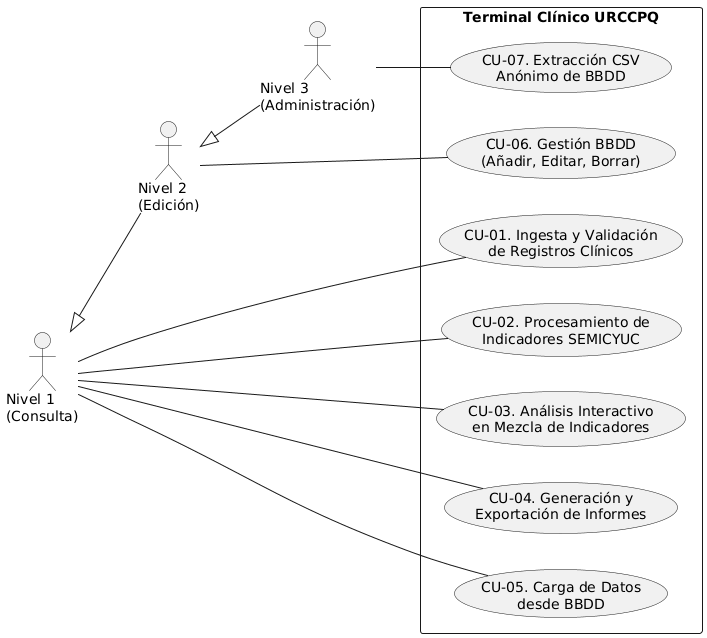
\includegraphics[width=0.7\textwidth]{img/uml.png}
    \caption{Diagrama \textit{UML} del proyecto.}
    \label{fig:uml}
\end{figure}

\section{Explicación casos de uso.}
Las \textbf{tablas de explicación de casos de usos} \cite{tablas_casos} sirven para detallar el funcionamiento de un sistema, yendo más allá del diagrama gráfico para definir el flujo paso a paso, actores, condiciones y excepciones. Son cruciales en la fase de análisis para asegurar que desarrolladores y clientes tengan la misma visión antes de programar, facilitando la creación de pruebas. 

\subsection{Requisitos}
Los requisitos funcionales describen el comportamiento esperado del \textit{software} frente a las interacciones del facultativo y las necesidades de procesamiento de datos clínicos.

\begin{itemize}
    \item \textbf{RF-01:} El sistema debe permitir la carga de archivos de monitorización clínica desde el almacenamiento local del dispositivo.
    \item \textbf{RF-02:} El sistema debe validar estructuralmente los datos de entrada, requiriendo estrictamente formato \textit{.csv} y limitando la ingesta a un máximo de 10 archivos simultáneos para prevenir desbordamientos de memoria.
    \item \textbf{RF-03:} El sistema debe integrar un motor algorítmico capaz de procesar la información y calcular los indicadores de calidad y seguridad definidos por la \textit{SEMICYUC}.
    \item \textbf{RF-04:} El sistema debe proveer un cuadro de mandos (\textit{dashboard}) interactivo que renderice los resultados matemáticos mediante gráficos lineales y de barras.
    \item \textbf{RF-05:} El sistema debe habilitar una herramienta de mezcla visual que permita la superposición paramétrica de hasta tres indicadores estadísticos para su análisis comparativo cruzado.
    \item \textbf{RF-06:} El sistema debe facultar la exportación de la sesión clínica, permitiendo empaquetar y descargar los cálculos y reportes generados al disco duro local.
    \item \textbf{RF-07:} El sistema debe implementar un modelo de \textbf{Control de Acceso Basado en Roles (\textit{RBAC})}, definiendo y restringiendo operativamente los niveles de visualización (Nivel 1), edición clínica (Nivel 2) y administración (Nivel 3).
    \item \textbf{RF-08:} El sistema debe permitir la consulta y carga de registros clínicos directamente desde la base de datos relacional (\textit{PostgreSQL}) hacia la memoria volátil de la aplicación, habilitando el análisis del histórico para todos los niveles de usuario.
    \item \textbf{RF-09:} El sistema debe exigir obligatoriamente la ejecución de una búsqueda previa de pacientes en la base de datos, evaluando su preexistencia antes de habilitar cualquier acción de modificación.
    \item \textbf{RF-10:} El sistema debe facultar a los usuarios con privilegios de Nivel 2 o superior para gestionar activamente la información, permitiendo añadir nuevos registros, así como editar o borrar pacientes existentes asegurando la integridad referencial.
    \item \textbf{RF-11:} El sistema debe autorizar exclusivamente a los administradores (Nivel 3) a realizar extracciones masivas del histórico clínico desde la base de datos hacia formato \textit{CSV}, aplicando un proceso de anonimización algorítmico automático para garantizar el cumplimiento estricto de la \textit{LOPD}.
\end{itemize}

\subsection{Requisitos de \textit{Hardware} y Autonomía}
Para garantizar la operabilidad del terminal en los distintos boxes de la unidad de Reanimación, se han definido los siguientes requisitos físicos y de gestión energética:

\begin{itemize}
    \item \textbf{RF-12 (Autonomía Energética):} El dispositivo debe ser completamente autónomo, permitiendo el desplazamiento del facultativo sin dependencia de cables. Para ello, debe integrar una batería de polímero de litio (\textit{LiPo}\footnote{Es una batería recargable de alta densidad energética y peso ligero}) de gran capacidad (6000\textit{mAh} a 3.7\textit{V}).
    \item \textbf{RF-13 (Gestión de Carga e Interrupción):} El sistema debe incorporar un módulo de gestión de energía (\textit{Adafruit PowerBoost 1000C}) que permita la recarga de la batería mediante un puerto \textit{Micro-USB} y garantice un flujo estable de 5.2\textit{V} a la \textit{Raspberry Pi}, incluso durante el proceso de carga (\textit{load-sharing}\footnote{Es una técnica de gestión de energía que permite a un dispositivo electrónico funcionar utilizando la energía de la fuente externa mientras simultáneamente carga su batería.}).
    \item \textbf{RF-14 (Protección Física y Fabricación Aditiva):} Todos los componentes electrónicos (placa, batería, gestor de carga y cableado) deben estar protegidos por una carcasa diseñada a medida y fabricada mediante impresión \textit{3D}, asegurando el aislamiento eléctrico y la ventilación pasiva de los componentes.
    \item \textbf{RF-15 (Control de Alimentación Manual):} El terminal debe disponer de un interruptor físico conectado al pin \textit{Enable} del gestor de carga para permitir el encendido y apagado completo del sistema, evitando el drenaje innecesario de la batería cuando no esté en uso.
\end{itemize}

\subsection{Requisitos No Funcionales (RNF)}
Los requisitos no funcionales establecen las métricas de calidad, rendimiento, ergonomía y seguridad que condicionan el diseño de la arquitectura.

\begin{itemize}
    \item \textbf{RNF-01 (Seguridad y Privacidad):} Dada la sensibilidad de los datos procesados, el sistema debe operar de manera aislada (\textit{web} local en la \textit{Raspberry Pi} y despliegue en la \textit{intranet} del \textit{HUBU}), asegurando que ningún historial clínico sea transmitido a redes externas o servicios en la nube.
    \item \textbf{RNF-02 (Ergonomía y Usabilidad):} La interfaz gráfica (\textit{UI}) debe ser completamente \textit{responsive} y sus elementos de interacción (botones, selectores) deben estar dimensionados y optimizados para el uso en máquina de sobremesa o en la pantalla táctil de 7 pulgadas del terminal.
    \item \textbf{RNF-03 (Rendimiento):} El tiempo de respuesta del motor matemático de \textit{Python} para el cálculo y renderizado de un indicador clínico no debe penalizar la agilidad del facultativo durante una urgencia médica.
\end{itemize}

A continuación se detallan las siete tablas desarrolladas para este proyecto:

\begin{itemize}
	\item La Tabla \ref{tab:1} desarrolla el proceso de carga y procesamiento de los datos.
	
\begin{table}[hbt!]	\centering
	\begin{tabularx}{\linewidth}{ p{0.21\columnwidth} p{0.71\columnwidth} }
		\toprule
		\textbf{CU-1}    & \textbf{Ingesta y Validación de Registros Clínicos}\\
		\toprule
		\textbf{Versión}              & 1.0    \\
		\textbf{Autor}                & Nicolás García Gómez \\
		\textbf{Requisitos asociados} & RF-01, RF-02 \\
		\textbf{Descripción}          & Proceso mediante el cual el usuario carga los archivos brutos y el sistema verifica su integridad y formato. \\
		\textbf{Precondición}         & El usuario debe disponer de los archivos de monitorización exportados en formato \textit{CSV}. \\
		\textbf{Acciones}             &
		\begin{enumerate}
			\def\labelenumi{\arabic{enumi}.}
			\item El usuario accede al módulo de carga.
			\item El usuario selecciona los archivos desde su almacenamiento local.
			\item El sistema evalúa la extensión y el volumen de los archivos.
			\item El sistema almacena los datos en la memoria \textit{RAM} y muestra un mensaje de éxito.
		\end{enumerate}\\
		\textbf{Postcondición}        & Los datos validados quedan listos para su procesamiento algorítmico. \\
		\textbf{Excepciones}          & \textbf{Formato inválido o exceso de archivos:} Si un archivo no es \textit{.csv} o se seleccionan más de 10, el sistema aborta la carga y muestra un error. \\
		\textbf{Importancia}          & Alta \\
		\bottomrule
	\end{tabularx}
	\caption{Especificación del Caso de Uso CU-1.}
	\label{tab:1}
\end{table}		
	
	\item La tabla \ref{tab:2} detalla el método de selección de indicadores individuales
	
\begin{table}[hbt!]	\centering
	\begin{tabularx}{\linewidth}{ p{0.21\columnwidth} p{0.71\columnwidth} }
		\toprule
		\textbf{CU-2}    & \textbf{Procesamiento de Indicadores \textit{SEMICYUC}}\\
		\toprule
		\textbf{Versión}              & 1.0    \\
		\textbf{Autor}                & Nicolás García Gómez \\
		\textbf{Requisitos asociados} & RF-03, RF-04 \\
		\textbf{Descripción}          & Interacción para la selección de métricas específicas y ejecución del motor matemático. \\
		\textbf{Precondición}         & Deben existir datos validados en la memoria volátil del sistema (Postcondición CU-1 o CU-5). \\
		\textbf{Acciones}             &
		\begin{enumerate}
			\def\labelenumi{\arabic{enumi}.}
			\item El usuario navega hasta el desplegable de selección de indicadores.
			\item El usuario selecciona un indicador de calidad clínica del menú.
			\item El motor de \textit{Python} procesa los registros buscando los cálculos correspondientes.
			\item El sistema presenta los datos estadísticos por pantalla.
			\item El sistema permite visualizar dos tipos de gráficos
		\end{enumerate}\\
		\textbf{Postcondición}        & El indicador estadístico queda calculado y listo para descargar sus cálculos. \\
		\textbf{Excepciones}          & \textbf{Datos insuficientes:} Si los registros cargados no contiene la columna requerida para ese indicador, el sistema notifica la imposibilidad del cálculo. \\
		\textbf{Importancia}          & Alta \\
		\bottomrule
	\end{tabularx}
	\caption{Especificación del Caso de Uso CU-2.}
	\label{tab:2}
\end{table}	
	
	\item La Tabla \ref{tab:3} desglosa el método que permite el análisis gráfico de hasta tres indicadores de forma conjunta. 
	
\begin{table}[hbt!]	\centering
	\begin{tabularx}{\linewidth}{ p{0.21\columnwidth} p{0.71\columnwidth} }
		\toprule
		\textbf{CU-3}    & \textbf{Análisis Interactivo en Mezcla de Indicadores}\\
		\toprule
		\textbf{Versión}              & 1.0    \\
		\textbf{Autor}                & Nicolás García Gómez \\
		\textbf{Requisitos asociados} & RF-05 \\
		\textbf{Descripción}          & Uso de las herramientas de visualización, filtrado y comparativa gráfica (\textit{Dashboard} entre indicadores). \\
		\textbf{Precondición}         & Deben existir datos validados en la memoria volátil del sistema (Postcondición CU-1 o CU-5). \\
		\textbf{Acciones}             &
		\begin{enumerate}
			\def\labelenumi{\arabic{enumi}.}
			\item El usuario utiliza la herramienta de ``Mezcla'' para superponer hasta 3 indicadores.
			\item El usuario selecciona el tipo de visualización.
			\item El sistema renderiza la gráfica en la interfaz interactiva.
			\item El sistema actualiza la gráfica en tiempo real.
		\end{enumerate}\\
		\textbf{Postcondición}        & La información se muestra de manera visual y comprensible para la toma de decisiones. \\
		\textbf{Excepciones}          & \textbf{Límite de superposición:} Si se intentan mezclar más de 3 indicadores, el sistema bloquea la acción para preservar la legibilidad. \\
		\textbf{Importancia}          & Media \\
		\bottomrule
	\end{tabularx}
	\caption{Especificación del Caso de Uso CU-3.}
	\label{tab:3}
\end{table}	
	
	\item La Tabla \ref{tab:4} explica todo el proceso relativo a la generación del resumen de los indicadores y su descarga en forma de informe \textit{PDF}.
	
\begin{table}[hbt!]	\centering
	\begin{tabularx}{\linewidth}{ p{0.21\columnwidth} p{0.71\columnwidth} }
		\toprule
		\textbf{CU-4}    & \textbf{Generación y Exportación de Informes}\\
		\toprule
		\textbf{Versión}              & 1.0    \\
		\textbf{Autor}                & Nicolás García Gómez \\
		\textbf{Requisitos asociados} & RF-06 \\
		\textbf{Descripción}          & Empaquetado de los resultados y descarga en formatos estandarizados para la historia clínica. \\
		\textbf{Precondición}         & Deben existir datos validados en la memoria volátil del sistema (Postcondición CU-1 o CU-5). \\
		\textbf{Acciones}             &
		\begin{enumerate}
			\def\labelenumi{\arabic{enumi}.}
			\item El usuario pulsa el botón de descarga correspondiente al reporte deseado.
			\item El sistema recopila los cálculos y gráficas de la sesión actual.
			\item Se genera un archivo en formato estructurado (\textit{PDF} o tabla resumen).
			\item El archivo se descarga en el disco duro local del dispositivo.
		\end{enumerate}\\
		\textbf{Postcondición}        & El facultativo obtiene un documento físico/digital para archivar en el historial. \\
		\textbf{Excepciones}          & \textbf{Error de escritura:} Si el disco está lleno o no hay permisos, se alerta al usuario del fallo en la descarga. \\
		\textbf{Importancia}          & Alta \\
		\bottomrule
	\end{tabularx}
	\caption{Especificación del Caso de Uso CU-4.}
	\label{tab:4}
\end{table}

\item La Tabla \ref{tab:5} detalla el proceso de conexión y extracción de información clínica histórica directamente desde la \textit{BBDD}.
	
\begin{table}[hbt!]	\centering
	\begin{tabularx}{\linewidth}{ p{0.21\columnwidth} p{0.71\columnwidth} }
		\toprule
		\textbf{CU-5}    & \textbf{Carga de Datos desde BBDD}\\
		\toprule
		\textbf{Versión}              & 1.0    \\
		\textbf{Autor}                & Nicolás García Gómez \\
		\textbf{Requisitos asociados} & RF-07, RF-08 \\
		\textbf{Descripción}          & Consulta y extracción de registros clínicos desde \textit{PostgreSQL} hacia la memoria volátil del sistema para su análisis. \\
		\textbf{Precondición}         & El usuario debe tener acceso de Nivel 1 (o superior) y la base de datos debe estar operativa. \\
		\textbf{Acciones}             &
		\begin{enumerate}
			\def\labelenumi{\arabic{enumi}.}
			\item El usuario accede al módulo de interacción con la \textit{BBDD}.
			\item El usuario selecciona el año o rango de años a analizar.
			\item El sistema lanza una consulta estructurada a la base de datos.
			\item El sistema aloja los resultados en la memoria \textit{RAM} de la aplicación.
		\end{enumerate}\\
		\textbf{Postcondición}        & Los datos quedan listos en memoria para su procesamiento algorítmico (CU-2, CU-3 Y CU-4). \\
		\textbf{Excepciones}          & \textbf{Ausencia de años:} Si no se selecciona ningún  año, el sistema alerta al usuario y detiene la carga. \\
		\textbf{Importancia}          & Alta \\
		\bottomrule
	\end{tabularx}
	\caption{Especificación del Caso de Uso CU-5.}
	\label{tab:5}
\end{table}	

	\item La Tabla \ref{tab:6} expone las operaciones de administración directa sobre los registros clínicos, garantizando la integridad de la información.
	
\begin{table}[hbt!]	\centering
	\begin{tabularx}{\linewidth}{ p{0.21\columnwidth} p{0.71\columnwidth} }
		\toprule
		\textbf{CU-6}    & \textbf{Gestión BBDD (Añadir, Editar, Borrar)}\\
		\toprule
		\textbf{Versión}              & 1.0    \\
		\textbf{Autor}                & Nicolás García Gómez \\
		\textbf{Requisitos asociados} & RF-07, RF-09, RF-10 \\
		\textbf{Descripción}          & Módulo de administración para la inserción de nuevos pacientes y la modificación o eliminación de registros existentes. \\
		\textbf{Precondición}         & El usuario debe poseer credenciales de Nivel 2 (Edición Clínica) o superior. \\
		\textbf{Acciones}             &
		\begin{enumerate}
			\def\labelenumi{\arabic{enumi}.}
			\item El usuario accede al panel de gestión de registros.
			\item Si desea editar o borrar, el sistema exige realizar una búsqueda previa del paciente.
			\item El usuario introduce los nuevos datos o modifica los existentes en el formulario.
			\item El sistema ejecuta la transacción de escritura en \textit{PostgreSQL}.
		\end{enumerate}\\
		\textbf{Postcondición}        & La base de datos se actualiza manteniendo la consistencia de los historiales clínicos. \\
		\textbf{Excepciones}          & \textbf{Datos erróneos:} Si un usuario introduce datos sin sentido (ej. fecha de alta anterior a la de ingreso), el sistema bloquea la operación por seguridad. \\
		\textbf{Importancia}          & Alta \\
		\bottomrule
	\end{tabularx}
	\caption{Especificación del Caso de Uso CU-6.}
	\label{tab:6}
\end{table}	

	\item La Tabla \ref{tab:7} describe el flujo de exportación masiva y el proceso de protección de datos personales antes de su almacenamiento externo.
	
\begin{table}[hbt!]	\centering
	\begin{tabularx}{\linewidth}{ p{0.21\columnwidth} p{0.71\columnwidth} }
		\toprule
		\textbf{CU-7}    & \textbf{Extracción CSV Anónimo de BBDD}\\
		\toprule
		\textbf{Versión}              & 1.0    \\
		\textbf{Autor}                & Nicolás García Gómez \\
		\textbf{Requisitos asociados} & RF-07, RF-11 \\
		\textbf{Descripción}          & Exportación en formato \textit{CSV} del histórico clínico aplicando algoritmos de anonimización y borrado de identificadores personales. \\
		\textbf{Precondición}         & El usuario debe poseer credenciales exclusivas de Nivel 3 (Administración). \\
		\textbf{Acciones}             &
		\begin{enumerate}
			\def\labelenumi{\arabic{enumi}.}
			\item El administrador accede a la interfaz de la \textit{BBDD}, habilitándose el botón especifico de exportación.
			\item El sistema recupera el volumen de datos solicitado desde \textit{PostgreSQL}.
			\item El motor de la aplicación purga automáticamente la columna identificativa (Número de Historia Clínica).
			\item Se empaqueta la información resultante en un archivo \textit{CSV}.
			\item El sistema descarga el archivo anonimizado en el dispositivo local.
		\end{enumerate}\\
		\textbf{Postcondición}        & Se obtiene un conjunto de datos legales aptos para investigación o auditoría externa. \\
		\textbf{Excepciones}          & \textbf{Ausencia de años:} Si no se selecciona ningún  año, el sistema alerta al usuario y detiene la carga. \\
		\textbf{Importancia}          & Alta \\
		\bottomrule
	\end{tabularx}
	\caption{Especificación del Caso de Uso CU-7.}
	\label{tab:7}
\end{table}	
\end{itemize}

\section{Prototipos de interfaz o interacción con el proyecto}
En el desarrollo de \textit{software} con aplicación clínica, el diseño de la \textbf{experiencia de usuario} (\textit{UX}) y la \textbf{interfaz de usuario} (\textit{UI}) es tan crítico como el propio motor algorítmico. Una interfaz mal diseñada en un entorno de alta presión como una unidad de Reanimación (\textit{URCCPQ}) puede inducir a errores operativos o retrasar la toma de decisiones. 

Por ello, de forma previa a la codificación de las vistas en el \textit{framework Reflex}, se ha llevado a cabo una fase de prototipado de baja fidelidad (\textit{wireframing}). Esta práctica es un estándar en la ingeniería de \textit{software} porque permite:
\begin{itemize}
    \item Definir la distribución espacial de la información minimizando la carga cognitiva del facultativo.
    \item Detectar de forma temprana problemas de usabilidad o cuellos de botella en la navegación.
    \item Validar que la disposición de los elementos (botones, selectores, gráficas) se ajusta a los requisitos ergonómicos de las unidades computacionales de la \textit{URCCPQ} y de una pantalla táctil de 7 pulgadas.
\end{itemize}

A continuación, se presentan los prototipos estructurales de las siete vistas fundamentales que componen la arquitectura visual del terminal:

\begin{itemize}
    \item \textbf{Pantalla Principal de Ingesta (Figura \ref{fig:web_inicio}):} Representa la vista inicial del sistema. Su diseño es minimalista, centrando la atención del usuario en el área de carga (arrastrar y soltar) para los archivos \textit{.csv} de monitorización o la apertura de la base de datos, cumpliendo con el Caso de Uso CU-01.
    
    \begin{figure}[h]
		\centering
    		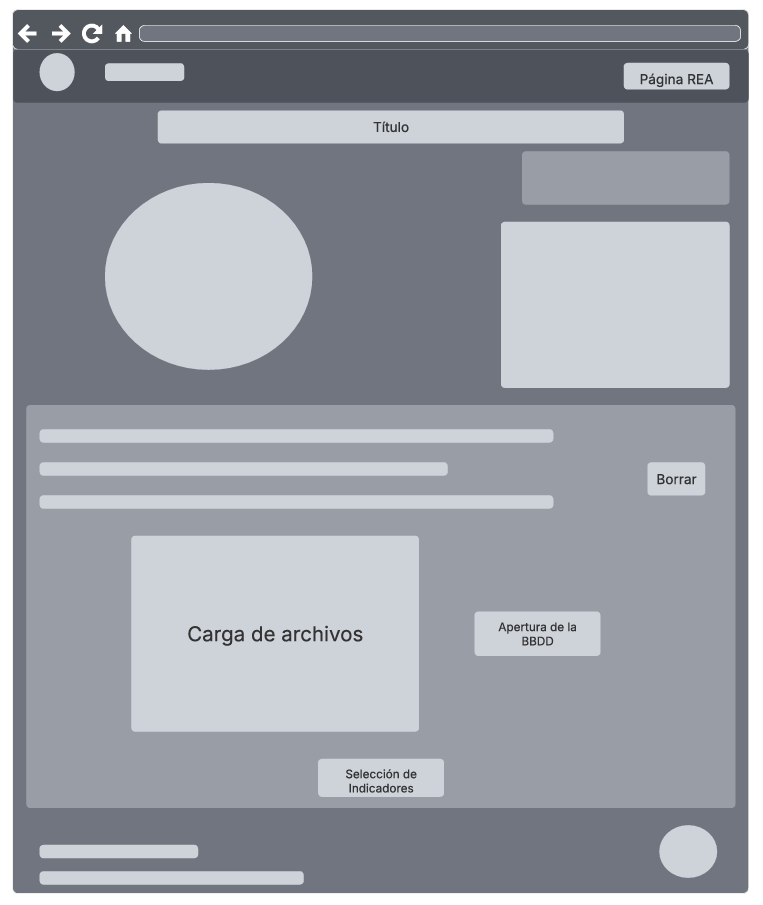
\includegraphics[width=0.85\textwidth]{img/web_inicio.png}
    		\caption{Pantalla principal de la \textit{web}.}
    		\label{fig:web_inicio}
	\end{figure}

    
    \item \textbf{Menú de Navegación y Enrutamiento (Figura \ref{fig:web_seleccion}):} Muestra la disposición del panel de control lateral o desplegable, diseñado con una tipografía y áreas de pulsación amplias para facilitar el salto rápido entre los distintos módulos analíticos sin requerir gran precisión.
    
    \begin{figure}[h]
		\centering
    		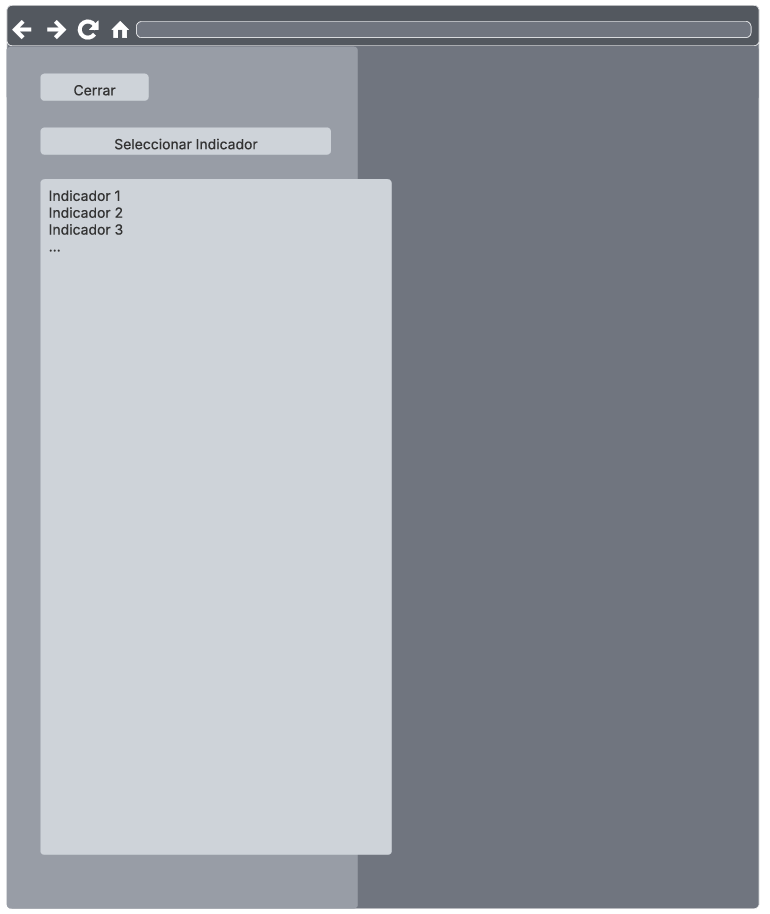
\includegraphics[width=0.85\textwidth]{img/web_seleccion.png}
    		\caption{Panel de selección lateral.}
    		\label{fig:web_seleccion}
	\end{figure}
    
    \item \textbf{Vista de Indicador Individual (Figura \ref{fig:web_indicador}):} Esboza la estructura del área de trabajo clínico. En la parte superior se ubican las métricas \textit{SEMICYUC} (CU-02), mientras que el cuerpo central está reservado para la renderización en gran formato de las gráficas (lineal o barras).
    
    \begin{figure}[h]
		\centering
    		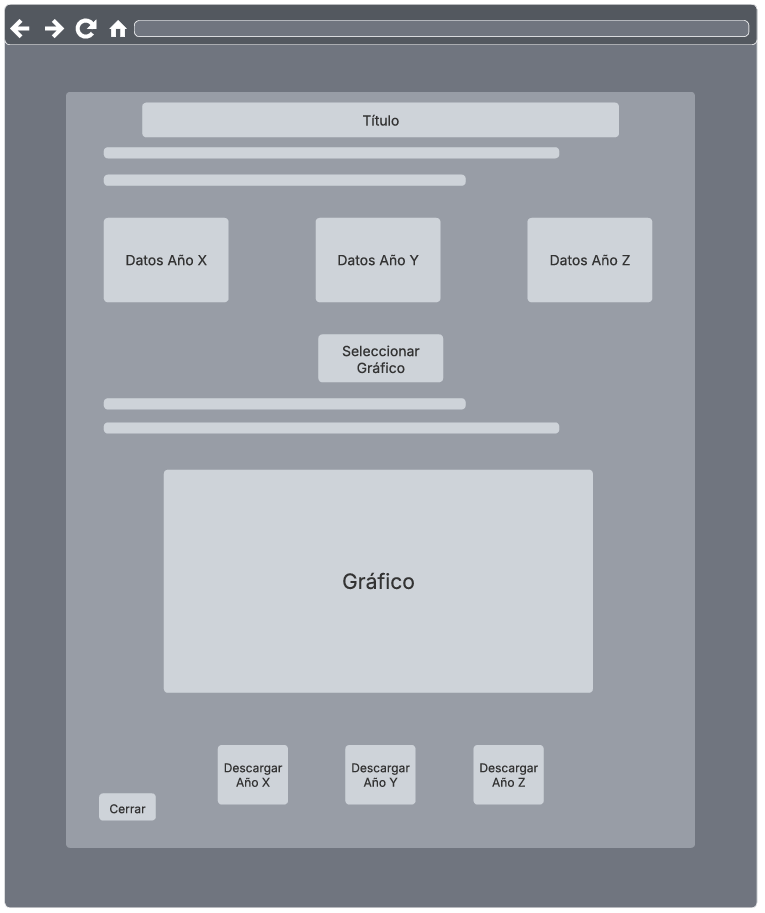
\includegraphics[width=0.85\textwidth]{img/web_indicador.png}
    		\caption{Indicador individual.}
    		\label{fig:web_indicador}
	\end{figure}
    
    \item \textbf{Herramienta de Mezcla y Comparativa (Figura \ref{fig:web_mezcla}):} Este prototipo ilustra la funcionalidad más avanzada del sistema. Muestra cómo el facultativo puede añadir iterativamente hasta tres indicadores, visualizando la leyenda cruzada y la superposición de datos en el lienzo principal (CU-03).
    
    \begin{figure}[h]
		\centering
    		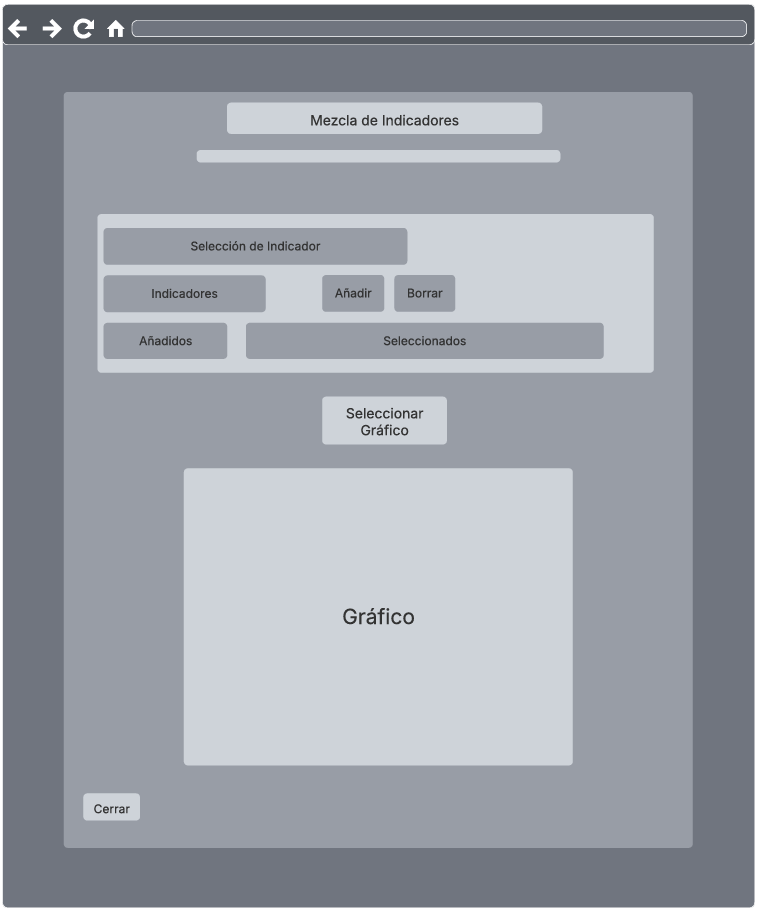
\includegraphics[width=0.85\textwidth]{img/web_mezcla.png}
    		\caption{Mezcla de indicadores.}
    		\label{fig:web_mezcla}
	\end{figure}
    
    \item \textbf{Panel de Resumen Global (Figura \ref{fig:web_resumen}):} Representa el cuadro de mandos final, donde se agrupan las métricas totales y la distribución por especialidades en formato tabular. Incluye los botones de acción (\textit{Call to Action o \textit{CTA}}) para la generación y exportación del informe final en \textit{PDF} (CU-04).
    
	\begin{figure}[h]
		\centering
    		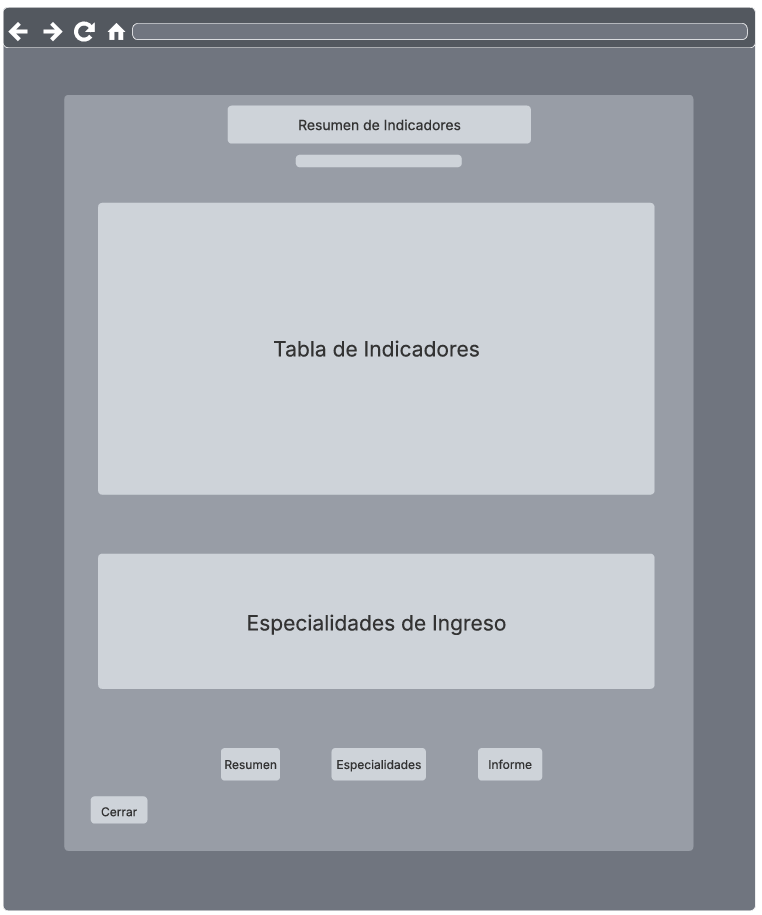
\includegraphics[width=0.85\textwidth]{img/web_resumen.png}
    		\caption{Resumen final de los indicadores.}
    		\label{fig:web_resumen}
	\end{figure}    
    
    \item \textbf{Pantalla de Inicio de Sesión (Figura \ref{fig:web_acceso}):} Representa el portal de autenticación seguro de la aplicación. Su diseño diferencia claramente dos áreas de entrada: un bloque principal destinado al acceso clínico habitual mediante correo y contraseña (Niveles 1, 2 y 3), y una sección inferior reservada exclusivamente para el acceso administrativo (Nivel 3). Esta pasarela es indispensable para garantizar la trazabilidad y asignar dinámicamente los módulos disponibles según el modelo jerárquico implementado.
    
    \begin{figure}[h]
		\centering
    		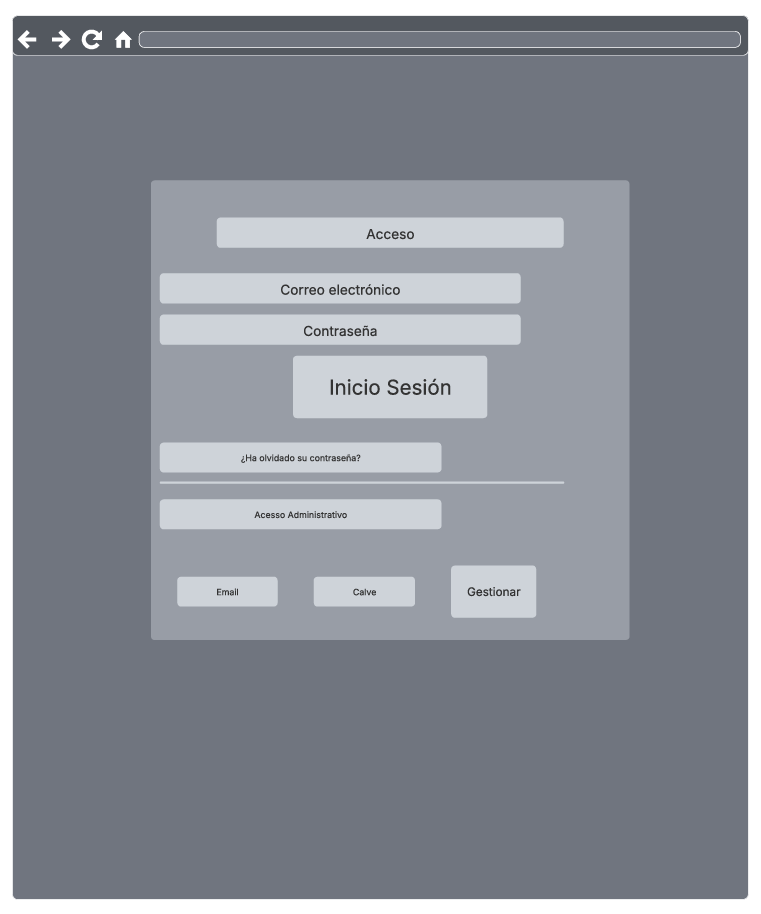
\includegraphics[width=0.85\textwidth]{img/web_acceso.png}
    		\caption{Pantalla de inicio de sesión y validación de roles.}
    		\label{fig:web_acceso}
	\end{figure}

    \item \textbf{Interfaz de la Base de Datos (Figura \ref{fig:web_bbdd}):} Ilustra el panel unificado de gestión clínica. Su diseño modulariza visualmente las funciones según los casos de uso: el bloque superior gestiona la selección por años (CU-05); el bloque central contiene los campos de búsqueda por número de historia para habilitar la adición, edición o borrado de pacientes (CU-06); y la barra inferior agrupa las acciones globales, destacando la carga a la memoria de la aplicación y el botón de exportación (CU-07), el cual solo será funcional si el rol del usuario lo permite.
    
    \begin{figure}[h]
		\centering
    		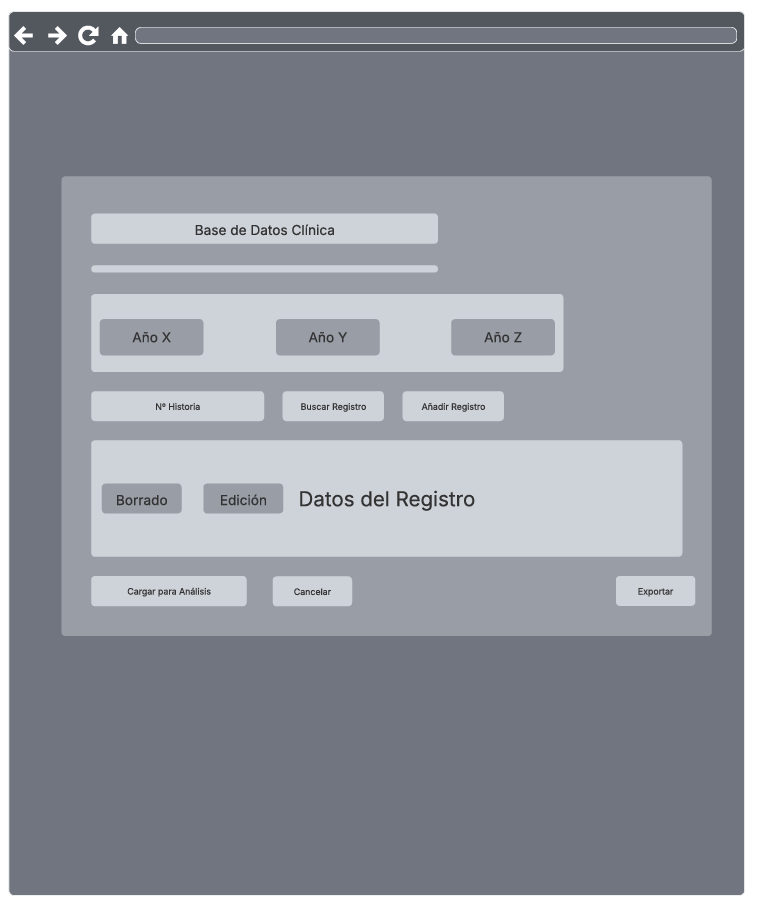
\includegraphics[width=0.85\textwidth]{img/web_bbdd.png}
    		\caption{Interfaz unificada para la gestión y consulta de la \textit{BBDD}.}
    		\label{fig:web_bbdd}
	\end{figure}
\end{itemize}



